\documentclass[12pt,compress,aspectratio=169]{beamer}

\usetheme{metropolis}
\setbeamersize{text margin left=.5cm,text margin right=.5cm}

%  \setbeamertemplate{navigation symbols}{} % suppress nav bar
%  \setbeamercovered{transparent}

\usefonttheme{professionalfonts}
\usepackage{graphicx}
\usepackage{tikz}
\usepackage{amsmath}
\usepackage{mathpazo}
%\usepackage[scaled]{helvet}
\usepackage{xcolor,colortbl}
\usepackage{hyperref}
\usepackage{siunitx}

\setmonofont{Ubuntu Mono}
\setlength{\parskip}{0pt}
\renewcommand{\baselinestretch}{1}


\sisetup{
  number-math-rm=\mathnormal,
  per-mode=symbol
}

\title{Topic 21: Special Relativity}
\subtitle{Advanced Placement Physics}
\author[TML]{Dr.\ Timothy Leung}
\institute{Olympiads School\\Toronto, Ontario, Canada}
\date{April 2020}



\newcommand{\mb}[1]{\mathbf{#1}}
\newcommand{\pic}[2]{\includegraphics[width=#1\textwidth]{#2}}
\newcommand{\bigsqrt}{\ensuremath\sqrt{1-\left(\frac{v}{c}\right)^2}}
\newcommand{\lorentz}{\ensuremath\frac{1}{\bigsqrt}}
\newcommand{\eq}[2]{\vspace{#1}{\Large\begin{displaymath}#2\end{displaymath}}}



\begin{document}

\begin{frame}
  \maketitle
\end{frame}

%
%
%\section[Intro]{Introduction}
%
%\begin{frame}{Introduction}
%  These slides for this topic are an expanded version of the slides used for
%  Grade 12 Physics (with some additional calculus). There are two versions of
%  the slides; both are downloadable from the school website:
%  \begin{itemize}
%  \item The long version
%    \begin{itemize}
%    \item More background information (more than needed for the AP 2 Exam) and
%      derivations and integrations
%    \item May answer some of your questions about the specifics of the theory
%    \item \texttt{21-relativity-long.pdf}
%    \end{itemize}
%  \item The short version
%    \begin{itemize}
%    \item More ``to the point''
%    \item The version that is used during class
%    \item \texttt{21-relativity-short.pdf}
%    \end{itemize}
%  \end{itemize}
%  There is also a handout on how to solve and interpret the time dilation
%  problem
%\end{frame}


\section{Reference Frame}

\begin{frame}{Frame of Reference}
  You can think of a \textbf{frame of reference} (or ``reference frame'', or
  just ``frame'') as a hypothetical mobile ``laboratory'' an observer uses to
  make measurements (e.g.\ mass, lengths, time). At a minimum, it includes:
  \begin{itemize}
  \item Some rulers (i.e.\ coordinate system) to measure  positions and lengths
  \item A clock to measure the passage of time
  \item A scale to compare forces
  \item A balance to measure masses
  \end{itemize}
  \vspace{.15in}\textcolor{red!85}{High-school textbooks often refer to the
    frame of reference as a ``coordinate system''. While it certainly includes
    that, this definition often makes it difficult to understand special
    relativity.}
\end{frame}



\begin{frame}{Frame of Reference}
  \begin{itemize}
  \item We assume that the hypothetical laboratory is \emph{perfect}---all the
    hypothetical ``instruments'' have zero errors
  \item What matters is the \emph{motion} (at rest, uniform motion, acceleration
    etc) of your laboratory, and how it affects the measurement that you make
  \item ``From the point of view of\ldots''
  \end{itemize}
\end{frame}


\begin{frame}{Inertial Frame of Reference}
  An \textbf{inertial frame of reference} (or a \textbf{rest frame}) is one
  that is moving in uniform motion
  \begin{itemize}
  \item In an inertial frame, Newton's first and second laws of motion are valid
  \item Since all uniform motion are treated the same way, you may consider
    any inertial frames of reference to be \emph{at rest}
  \end{itemize}
  \vspace{.2in}
  \begin{block}{The Principle of Relativity}
    All laws of motion must apply equally in all inertial frames of reference.
  \end{block}
\end{frame}



\begin{frame}{Inertial Frame of Reference}
  Observer A moves uniformly with the skateboard, while Observer B stands on
  the side of the road. So, when A tosses a ball upward:
  \begin{center}
    \pic{.55}{graphics/57.png}
  \end{center}
  \begin{itemize}
  \item A sees only vertical motion, while
  \item B sees the ball traveling in a parabolic curve, although
  \item A \& B observe different motion, but they agree on the \emph{equations}
    that govern the motion
  \end{itemize}
\end{frame}



\begin{frame}{Inertial Frame of Reference}
  Observer A sees the same motion (only vertical motion) regardless of whether
  he is moving uniformly w.r.t.\ B or not (as long as \emph{neither} are
  accelerating)
  \begin{center}
    \pic{.55}{graphics/57.png}
  \end{center}
  \begin{itemize}
  \item Valid for A to conclude that he is at rest, but that B and the rest of
    the world are moving
  \item Likewise, it is also valid for B to think that he is at rest, but it is
    only A and his skateboard that are moving
  \end{itemize}
\end{frame}
    

\begin{frame}{Newtonian (Classical) Relativity}
  When studying kinematics and dynamics, we made some untested assumptions that
  seemed obvious: space and time are \emph{absolute}
  \begin{itemize}
  \item \SI{1}{m} is \SI{1}{m} no matter where you are, or how you are moving
  \item \SI{1}{s} is \SI{1}{s} no matter where you are, or how you are moving
  \item Measurements of space and time do not depend on motion
  \end{itemize}
  \vspace{.1in}If space and time are absolute, then \emph{all} velocities are
  relative to the observer
  \begin{itemize}
  \item Measured velocities depend on the motion of the observer
  \item Galilean velocity addition rule:

    \eq{-.25in}{
      \boxed{\mb{v}_{AC}=\mb{v}_{AB}+\mb{v}_{BC}}
    }
  \end{itemize}
\end{frame}


%\begin{frame}{New Physics: Maxwell's Equations}
%  \begin{columns}
%    \column{0.3\textwidth}
%    \begin{center}
%      \pic{1}{graphics/PORTRAIT-James-Clerk-Maxwell.jpg}\\
%      James Clerk Maxwell
%    \end{center}
%    \column{0.7\textwidth}
%    \begin{itemize}
%    \item Classical laws of electrodynamics
%    \item Published in 1861 and 1862
%    \item Explains the relationship between
%      \begin{itemize}
%      \item Electricity
%      \item Electric Circuits
%      \item Magnetism
%      \item Optics
%      \end{itemize}
%    \item Previously these disciplines are thought to be separate and not
%      related
%    \end{itemize}
%  \end{columns}
%\end{frame}


\begin{frame}{Maxwell's Equations}
  Maxwell's equations on electrodynamics in a vacuum (studied previously):
  
  \vspace{-.35in}{\Large
    \begin{align*}
      \nabla\cdot\mb{E} &= 0\\
      \nabla\cdot\mb{B} &= 0\\
      \nabla\times\mb{E} &=-\frac{\partial\mb{B}}{\partial t}\\
      \nabla\times\mb{B} &=\mu_0\varepsilon_0\frac{\partial\mb{E}}{\partial t}
    \end{align*}
  }
  
  \vspace{-.1in}Disturbances in $\mb{E}$ and $\mb{B}$ travel as an
  \emph{electromagnetic wave} with a speed $c$:

  \vspace{-.25in}{\Large
    \begin{displaymath}
      c=\frac{1}{\sqrt{\varepsilon_0\mu_0}}=\SI{299792458}{m/s}
    \end{displaymath}
  }
\end{frame}


\begin{frame}{Peculiar features of Maxwell's equation}
  \begin{itemize}
  \item Does not mention the \emph{medium} in which EM waves travels
  \item When applying \emph{Galilean transformation} (from which we obtain
    the velocity addition rule) to Maxwell's equations, asymmetry is introduced
  \item Gauss's law for magnetism break down: magnetic field lines appear to
    have beginnings/ends
  \item In \emph{some} inertial frames of reference, Maxwell's equations are
    simple and elegant, but transform the equation into another inertial frame,
    the equations are ugly and complex!
  \item Physicists at the time began to theorize that (perhaps) there is an
    actual \emph{preferred} inertial frame of references
  \item This seems to violate the \emph{principle of relativity}
  \end{itemize}
\end{frame}



\begin{frame}{The Illusive Ether}
  Maxwell's hypothesis: the speed of light $c_0$ is relative to a hypothetical
  subtance called \textbf{luminiferous aether} (or just \textbf{ether}) that
  permeates the universe. Ether must have some fantastic properties:
  \begin{itemize}
  \item All space is filled with ether
  \item Massless
  \item Zero viscosity
  \item Non-dispersive
  \item Incompressible
  \item Continuous at a very small (sub-atomic) scale
  \end{itemize}
  It was thought that the preferred inertial reference frame is that of the
  ether
\end{frame}



\begin{frame}{Spoiler Alert}
  Spoiler alert: Ether doesn't exist.
\end{frame}



\begin{frame}{The Michelson-Morley Experiment}
  If ether exists, then at different times of the year, the Earth will have a
  different relative velocity with respect to it:
  \begin{center}
    \pic{.35}{graphics/2000px-AetherWind.png}
  \end{center}
  And it causes light to speed up or slow down. By measuring and comparing the
  speed of light at various times of the year, we should be able to determine
  to flow of ether relative to Earth.
\end{frame}



\begin{frame}{Michelson-Morley Experiment}
  American phycisists Albert Michelson\footnote{Nobel Prize in Physics, 1907}
  and Edward Morley designed an ingenious but very difficult experiment to
  detect ether using an \textbf{interferometer} designed by Michelson
  \begin{center}
    \pic{.7}{graphics/michelsonmorley.jpg}
  \end{center}
\end{frame}



\begin{frame}{The Michelson Interferometer}
  \begin{columns}
    \column{.3\textwidth}
    \begin{center}
      \pic{1.15}{graphics/313754.png}
    \end{center}

    \column{.7\textwidth}
    \begin{itemize}
    \item A beam of light is split into two using a two-way (half-silvered)
      mirror
    \item The two beams are reflected off mirrors and finally arriving at the
      screen where interference patterns are observed
    \item The two paths are the same length, so if the \emph{speed} of the light
      changes, we should see an interference pattern
    \item\textbf{Except none were ever found!} The interference patterns that
      could be observed were well within experimental errors, and far below
      expected values
    \end{itemize}
  \end{columns}
\end{frame}



\begin{frame}{What To Do with ``Null Result''}
  The Michelson-Morley experiment failed to detect the flow of ether, even
  after many refinements. What does this mean?
  \begin{itemize}
  \item Majority view
    \begin{itemize}
    \item\textbf{The experiment was flawed!} It is actually a reasonable
      guess, since the experiment is known to be a difficult one, errors can
      be introduced
    \item Keep improving the experiment (or design a better experiment) and
      Earth's motion relative to ether will eventually be found
    \end{itemize}
  \item Minority view:
    \begin{itemize}
    \item\textbf{The ether hypothesis is wrong!}
    \item The experiment showed it for what it is: ether either cannot be
      detected or it doesn't exist
    \end{itemize}
  \item A few physicists: The must be \textbf{another explanation} that saves
    both experiment and theory
  \end{itemize}
\end{frame}



\begin{frame}{Hendrik Lorentz}
%  \begin{columns}
%    
%    \column{.17\textwidth}
%    \begin{center}
%      \pic{1.2}{graphics/lorentz.jpg}\\
%          {\footnotesize Hendrik Lorentz}
%    \end{center}
%    
%    \column{.83\textwidth}
  Dutch physicist Hendrik Antoon Lorentz\footnote{1853--1928, Nobel Prize in
    Physics, 1902} was one of the first to consider the findings of
  Michelson-Morley experiment to be significant
  \begin{itemize}
  \item Lorentz's hypothesis: objects traveling in the direction of ether must
    contract in length, nullifying the experimental results
  \item The length contraction is given by the \textbf{Lorentz factor}:
    
    \eq{-.2in}{
      \boxed{\gamma=\lorentz}
    }
  \item But \emph{No known physical phenomenon} causes an object to contract
  \end{itemize}
%  \end{columns}
\end{frame}



\begin{frame}{Strange Behavior in Absolute Space Time}
  French mathematician Henri Poincar\'{e} also hypothesized that ether affects
  the flow of time the direction of motion. His equation is similar to the
  hypothesis by Lorentz and contains the same factor:

  \eq{-.2in}{
    \boxed{t' =\frac{t}{\bigsqrt}}
  }
  
  But \emph{no known physical phenomenon} can alter the flow of time either!

  \uncover<2>{
    \vspace{.15in}Both Poincar\'{e} and Lorentz depended their hypothesis on
    \begin{itemize}
    \item Absolute time and space
    \item Existence of ether
    \end{itemize}
  }
\end{frame}



\begin{frame}{Making Maxwell's Equations Work}
  \begin{columns}
    \column{.2\textwidth}
    \pic{1.1}{graphics/Einstein_patentoffice.png}
    \begin{center}
      \vspace{-.15in}{\footnotesize Albert Einstein\\ in 1905\par}
    \end{center}
    
    \column{.8\textwidth}
    \begin{itemize}
    \item In 1905, at the age of 26, Albert Einstein was working as a patent
      clerk in Bern, Switzerland while completing his Ph.D.
      \begin{itemize}
      \item Believed in the principle of relativity, and therefore
      \item Rejected the concept of a ``preferred'' frame of reference
      \end{itemize}
    \item The failure of the Michelson-Morley experiment to find the flow of
      ether proves that it does not exist
    \item In order to make Maxwell's equations to work again, Einstein
      revisited two most fundamental concepts in physics: \emph{space} and
      \emph{time}
    \end{itemize}
  \end{columns}
\end{frame}


\begin{frame}{Special Relativity}
  Published in \emph{Annalen der Physik} on September 26, 1905 in the article
  \emph{On the Electrodynamics of Moving Bodies}
  \begin{itemize}
  \item Submitted on June 30, 1905 and passed for publication by a referee
  \item Einstein's third paper (of four) that year
  \item Mentions only five other scientists by name: Issac Newton, James
    Clerk Maxwell, Heinrich Hertz, Christian Doppler and Hendrik Lorentz, but
    does not contain references to any publications
  \item Ignored by most physicists at first, until Max Planck took interests
  \item Called ``special relativity'' because it describes a ``special case''
    without effects of gravity
  \end{itemize}
\end{frame}



\begin{frame}{Postulates of Special Relativity}
  \begin{block}{The Principle of Relativity}
    \emph{All} laws of physics must apply equally in \emph{all} inertial frames
    of reference.
  \end{block}
  \begin{itemize}
  \item Reaffirms the principle in which physics is based on
  \item Extends the principle to include electrodynamics%(Maxwell's equations)
  \end{itemize}

  \vspace{.1in}
  \begin{block}{The Principle of Invariant Light Speed}
    As measured in any inertial frame of reference, light always propagates in
    empty space with a definite velocity $c_0$, independent of the state of
    motion of the emitting body.
  \end{block}
  \begin{itemize}
  \item Reaffirms the results from Michelson-Morley experiment
  \item Disproves the existence of ether
  \end{itemize}
%\end{frame}
%
%\begin{frame}
%  \frametitle{Postulates of Special Relativity}
  \vspace{.1in}The two postulates are unremarkable by themselves, but when
  combined, the consequences are profound
\end{frame}



\begin{frame}{What's so Special About Special Relativity?}
  Classical (Newtonian) relativity:
  \begin{itemize}
  \item Space and time are absolute (invariant), therefore
  \item The speed of light must be relative to the observer
  \end{itemize}

  \vspace{.1in}Einstein's special relativity:
  \begin{itemize}
  \item The speed of light is absolute (invariant), therefore
  \item Space and time must be relative to the observer
  \end{itemize}

  \vspace{.1in}We must modify our traditional concepts:
  \begin{itemize}
  \item Measurement of \emph{space}
  \item Measurement of \emph{time}
  \item Concept of \emph{simultaneity}
  \end{itemize}
\end{frame}



\section{Simultaneity}

\begin{frame}{The Relativity of Simultaneity}
  This \emph{thought experiment} is similar to the one that Einstein presented.
  Suppose lightning bolt strikes the two ends of a high-speed moving train.
  Does it happen simultaneously?
  \begin{center}
    \pic{.4}{graphics/87-1-1024x673.png}
  \end{center}

  \begin{itemize}
  \item\vspace{-.15in} Two \emph{independent} events: lightning striking the
    front, and lightning striking the back of the train
  \item The man on the ground sees the lightning bolt striking at the same time
  \item The woman on the moving train sees the lightning bolt on the front first
  \end{itemize}
\end{frame}



\begin{frame}{Relativity of Simultaneity}
  From the man's perspective:
  \begin{itemize}
  \item He is stationary, but the train is moving
  \item When the lightnings strike, he is at an equal distance from the front
    and the back of the train
  \item Flashes from the two lightning bolts arrive at his eyes at the same time
  \item Since the speed of light is a constant regardless of motion
  \end{itemize}
  Therefore, his conclusions are:
  \begin{itemize}
  \item The two lightnings must have happened at the same time
  \item The woman in the train made the wrong observation: she only
    \emph{thinks} that the lightning struck the front first because she is
    moving toward the light from the front
  \end{itemize}
\end{frame}


\begin{frame}{Relativity of Simultaneity}
  From the woman's perspective:
  \begin{itemize}
  \item\emph{She} is stationary, but the man and the rest of the world are
    moving
  \item When the lightnings strike, she is at an equal distance from the two
    ends of the train
  \item The flash from the front arrive first, then the back
  \item Since the speed of light is a constant regardless of motion
  \end{itemize}
  Therefore, her conclusions are:
  \begin{itemize}
  \item Lightnings must have struck the front first
  \item The man on the road made the wrong observation: he only \emph{thinks}
    that the lightning struck at the same time because he's moving toward the
    light from the back
  \end{itemize}
\end{frame}


\begin{frame}{Relativity of Simultaneity}
  \begin{itemize}
  \item The two observers disagree on the result, but
    \begin{itemize}
    \item Neither person is wrong
    \item Neither person is misinformed
    \end{itemize}
  \item Both observers are valid \emph{inertial} frames of reference, and
    therefore both can consider themselves at rest
  \item This means that \emph{simultaneity depends on your motion}
  \end{itemize}
  
  \vspace{.2in}\textbf{Relativity of Simultaneity: Events that are simultaneous
    in one inertial frame of reference are not simultaneous in another.}
\end{frame}



\section{Time Dilation}

\begin{frame}{Relativity of Time}
  \begin{center}
    \pic{.7}{graphics/spaceship.png}
  \end{center}

  \vspace{-.2in}While on a spaceship traveling through space, and I shine a
  light from $A$ (the bottom of my ship) to $B$ (at the top of my ship). The
  distance between $A$ and $B$ is:

  \eq{-.45in}{
      |AB|=ct
  }

  \vspace{-.2in}Knowing the speed of light $c$, and how long it takes for the
  light pulse to reach $B$, I can calculate the dimensions of my spaceship.
\end{frame}


\begin{frame}{Relativity of Time}
  \begin{center}
    \pic{.7}{graphics/spaceship.png}
  \end{center}
  Meanwhile, you are on a small planet watching my spaceship go past at speed
  $v$. You see that same beam of light travel from $A$ to $B'$ instead.
  \begin{center}
    \pic{.7}{graphics/light-a-b-prime.png}
  \end{center}
\end{frame}



\begin{frame}{Relativity of Time}
  We can relate the time interval of the beam of light observed by me (on the
  spaceship) and you (on the planet) using pythagorean theorem:
  \begin{center}
    \pic{.6}{graphics/dilation.png}
  \end{center}
  \begin{align*}
    c^2t'^2 &=v^2t'^2 + c^2t^2\\
    \left(c^2-v^2\right)t'^2 &=c^2t^2\\
    \left(1-\frac{v^2}{c^2}\right)t'^2 &=t^2\\
    t' &=\frac{t}{\bigsqrt}
  \end{align*}
\end{frame}


\begin{frame}{Relativity of Time}
  The relationship between observer is given by:
  
  \eq{-.2in}{
    \boxed{t' =\frac{t}{\bigsqrt}}
  }
  \begin{itemize}
  \item $t$ is called the \textbf{proper time}. It is the time measured
    by a person at rest relative to the object or event.
  \item $t'$ is called the \textbf{ordinary time} (aka \textbf{expanded time}
    or \textbf{dilated time}). It is the time measured by a moving observer in
    another inertial frame of reference. Since $v<c$, $t'$ is always greater
    than $t$.
  \end{itemize}
\end{frame}



\begin{frame}{Example Problem}
  \textbf{Example 1a:} Kim is riding a rocket that speeds past an asteroid at
  $v=0.600c$. If Kim sees \SI{10.}{\second} pass on her watch, how long would
  that time interval be as seen by Jim, an observer on the asteroid?

  \begin{displaymath}
    t' =\frac{t}{\bigsqrt}=\frac{10.0}{\sqrt{1-0.600^2}}=\SI{16.7}{\second}
  \end{displaymath}

  \uncover<2>{
    \begin{itemize}
    \item Jim observes that in the time it took Kim's clock to run
      \SI{10.}{\second}, his watch has already gone \SI{16.7}{\second},
      therefore
    \item Jim concludes that Kim's watch must be running slow
    \end{itemize}

    \textbf{Relativity of Time: A moving clock appears to run slow.}
  }
\end{frame}


\begin{frame}{Example Problem}
  \textbf{Example 1b:} Kim is riding a rocket that speeds past an asteroid at
  $0.600c$. If Jim, an observer in the \emph{asteroid}, sees \SI{10.}{\second}
  pass on his watch, how long would that time interval be as seen by Kim?

  \uncover<2>{
    \begin{displaymath}
      t' =\frac{t}{\bigsqrt}=\frac{10.0}{\sqrt{1-0.600^2}}=\SI{16.7}{\second}
    \end{displaymath}
    
    \begin{itemize}
    \item This problem is exactly the same as the last one!
    \item Kim observes that in the time it took Jim's clock to run
      \SI{10.}{\second}, her watch has already gone \SI{16.7}{\second},
      therefore
    \item Kim concludes that Jim's watch must be running slow
    \end{itemize}
  }
\end{frame}



\begin{frame}{How can that be?}
  How can the observer in the asteroid sees time in the rocket runs slowly,
  while the observer in the rocket \emph{also} sees time in the asteroid runs
  slowly?

  \vspace{.3in}\textbf{Answer:} the relativty of simultaneity. The clocks on the
  asteroid and on the rocket are \emph{not} synchronized.
  \begin{itemize}
  \item In example 1a, when Kim (on the rocket) starts measuring a
    \SI{10.}{\second} time interval, in order for Jim to compare that interval
    to \emph{his} watch, he has to start and end at the same time
    (simultaeously!) as Kim.
  \item But simultaneity is only relative. In Kim's reference frame, Jim never
    got the timing right!
  \item This problem reverses itself when Kim tries to synchronize her watch to
    Jim's \SI{10.}{\second} interval.
  \end{itemize}
\end{frame}


\section{Length Contraction}

\begin{frame}{Relativity of Space}
  Captain Quick is a comic book hero who can run at nearly the speed of light.
  In his hand, he is carrying a bomb set to explode in \SI{1.5}{\micro\second}.
  The bomb must be placed into its bracket before this happens. The distance
  ($L$) between the flare and the bracket is \SI{402}{\metre}.
  \begin{center}
    \vspace{-.15in}\pic{.7}{graphics/captain-quick.png}
  \end{center}
\end{frame}


\begin{frame}{Relativity of Space}
  Suppose Captain Quick runs at \SI{2.00e8}{\metre\per\second}, according to
  classical mechanics, he will not make it in time:
  \begin{displaymath}
    t= \frac{L}{v}=\frac{\SI{402}{\metre}}{\SI{2.00e8}{\metre\per\second}}
    =\SI{2.01e-6}{\second}=\SI{2.01}{\micro\second}
  \end{displaymath}
  But according to relativistic mechanics, he makes it just in time\ldots
\end{frame}


\begin{frame}{Relativity of Space}
  To a stationary observer, the time on the flare is slowed:
  \begin{displaymath}
    t'
    = \frac{t}{\bigsqrt}
    = \frac{\num{1.5e-6}}{\sqrt{1-\left(\frac{2.00}{3.00}\right)^2}}
    = \SI{2.01e-6}{\second}
  \end{displaymath}
  The stationary observer sees a passage of time of
  $t'=\SI{2.01}{\micro\second}$, but Captain Quick, who is in the same
  reference frame as the flare, experiences a passage of time of
  $t=\SI{1.50}{\micro\second}$, precisely the time for the flare to explode.
\end{frame}


\begin{frame}{Relativity of Space}
  If Captain Quick sees only $t=\SI{1.50}{\micro\second}$, then how far did he
  travel?
  \begin{itemize}
  \item Both Captain Quick and the observer on the side of the road agree that
    he is traveling at $v=\SI{2.00e8}{\metre\per\second}$
  \item The only possibility is that \emph{the distance actually got shorter}
    in Captain Quick's frame of reference, by this amount:
    
    \eq{-.2in}{
      \boxed{L'=L\bigsqrt}
    }
  \end{itemize}
  For this example:
  \begin{displaymath}
    L'=L\bigsqrt=402\sqrt{1-\left(\frac{2.00}{3.00}\right)^2}=\SI{300}{\metre}
  \end{displaymath}
\end{frame}


\begin{frame}{Length Contraction}
  Length contraction only occurs in the direction of motion
  \begin{center}
    \pic{.8}{graphics/baseball-contraction.jpg}
    \end{center}
\end{frame}

\begin{frame}{Example Problem}
  \textbf{Example 2:} A spacecraft passes Earth at a speed of \SI{2.00e8}{m/s}.
  If observers on Earth measure the length of the spacecraft to be
  \SI{554}{\metre}, how long would it be according to its passengers?
\end{frame}


\section{Lorentz Factor}

\begin{frame}{Lorentz Factor}
  The \textbf{Lorentz factor} $\gamma$ is a short-hand for writing length
  contraction, time dilation and relativistic mass:

  \eq{-.2in}{
    \boxed{\gamma=\lorentz}
  }
  
  Then time dilation and length contraction can be written simply as:
  
  \eq{-.1in}{
    \boxed{t' = \gamma t}\quad\boxed{L' = \frac{L}{\gamma}}
  }
\end{frame}


\begin{frame}{Summary}
  \begin{center}
    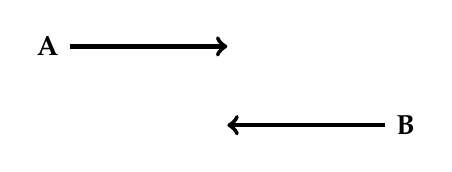
\begin{tikzpicture}[scale=2]
      \draw[ultra thick,->] (1,.5)--(2,.5) node[pos=0,left] {\textbf{A}};
      \draw[ultra thick,->] (3,0)--(2,0) node[pos=0,right]{\textbf{B}};
    \end{tikzpicture}
  \end{center}
  If observers A and B are moving at constant velocity relative to one another
  (doesn't matter if they're moving toward, or away from each other)
  \begin{itemize}
  \item They cannot agree whether any events happens at the same time or not
  \item Each sees the other's clock running slow
  \item Each sees the other ``contracted'' in length along the direction of
    motion
  \end{itemize}
\end{frame}


\begin{frame}{Lorentz Transformation}
  Time dilation and length contraction only tell part of the story. To account
  for the loss of simultaneity from one inertial frame to another, we need to
  use the \textbf{Lorentz transformation:}

  \vspace{-.45in}{\Large
    \begin{align*}
      x' &= \gamma(x-vt)\\
      y' &= y\\
      z' &= z\\
      t' &=\gamma\left(t-\frac{vx}{c^2}\right)
    \end{align*}
  }
  
  \vspace{-.1in}The Lorentz transformation ``solves'' many paradoxes
  (e.g.\ the twin paradox) from the time-dilation and
  length-contraction equations, but aren't really there.
\end{frame}



\begin{frame}{Lorentz Transformation}
  For slow speeds $v\ll c$, Lorentz transformation reduces to the Galilean
  transformation from classical mechanics, from which the velocity addition
  rule is formulated:

  \vspace{-.45in}{\Large
    \begin{align*}
      x' &= x-vt\\
      y' &= y\\
      z' &= z\\
      t' &= t'
    \end{align*}
  }
\end{frame}



\section{Rel.\ Velocity}

\begin{frame}{Relative Velocity}
  Unlike in classical mechanics, velocities (speeds) do not simply add. We have
  to account for time dilation and length contraction, which are included in
  the Lorentz transformation

  \vspace{.15in}\textbf{Einstein velocity addition rule}:

  \eq{-.2in}{
    \boxed{
      \mb{v}_{AC}=
      \frac{\mb{v}_{AB}+\mb{v}_{BC}}
           {1+\frac{\mb{v}_{AB}\cdot\mb{v}_{BC}}{c^2}}
    }
  }

  \vspace{.1in} If $v_{AB}\ll c$ and $v_{BC}\ll c$, we recover Galilean
  velocity addition rule
%  \item If the observer in frame $S$ measures an object moving along the
%    $x$-axis at velocity $u$, then the observer in the referenfe frame $S′$
%    that is moving at velocity $v$ in the $x$-direction with respect to $S$,
%    will measure the object moving with velocity $u′$:
%
%    \eq{-.2in}{
%      u'=
%      \frac{dx'}{dt'}=
%      \frac{\gamma(dx-vdt)}{\gamma(dt-vdx/c^2)}=
%      \frac{(dx/dt)-v}{1-(v/c^2)(dx/dt)}=
%      \frac{u-v}{1-uv/c^2}
%    }
%    
%  \item The other frame S will measure:
%    \eq{-.2in}{
%      u=
%      \frac{dx}{dt}=
%      \frac{\gamma(dx'+vdt')}{\gamma(dt'+vdx'/c^2)}=
%      \frac{(dx'/dt')+v}{1+(v/c^2)(dx'/dt')}=
%      \frac{u'+v}{1+u'v/c^2}
%    }
%  \end{itemize}
\end{frame}



\section{Relativistic Momentum}

\begin{frame}{Relativistic Momentum}
  In Grade 12 Physics, you were taught that momentum is mass times velocity.
  And in Grade 11 Physics, you were taught that velocity is displacement over
  time. \emph{These definitions have not changed.}

  \eq{-.2in}{
    \mb{p}=m\frac{d\mb{x}}{dt}
  }

  \vspace{-.1in}But now that you know $d\mb{x}$ and $dt$ are relativistic
  quantities that depend on motion, we can find a new expression for
  ``relativistic momentum'':
  
  \eq{-.2in}{
    \mb{p}=m\frac{d\mb{x}}{dt}
    =\frac{md\mb{x}}{\bigsqrt\;dt}
    =\boxed{\frac{m\mb{v}}{\bigsqrt}}=\gamma m\mb{v}
  }
\end{frame}


\section[Rel.\ Mass]{Relativistic Mass}

\begin{frame}{Relativistic Mass}
  From the relativistic momentum expression, we see the relativistic aspect to
  mass as well. The \textbf{apparent mass} (or \textbf{relativistic mass}) $m'$
  as measured by a moving observer is related to its \textbf{rest mass} (or
  \textbf{intrinsic mass} or \textbf{invariant mass}) $m$ by the Lorentz factor:

  \eq{-.18in}{
    \boxed{m'=\frac{m}{\bigsqrt}=\gamma m}
  }
  
  The intrinsic mass of a moving object does not change, but a moving observer
  will observe that it behaves as if it is more massive. As $v\rightarrow c$,
  $m'\rightarrow\infty$.
\end{frame}



\section[Energy]{Relativistic Energy}

\begin{frame}{Work and Energy}
  Einstein published a fourth paper in \emph{Annalen der Physik} on November
  21, 1905 (received Sept.\ 27) titled ``Does the Inertia of a Body Depend Upon
  Its Energy Content?'' (In German: Ist die Tr\"{a}gheit eines K\"{o}rpers von
  seinem Energieinhalt abh\"{a}ngig?)
  \begin{itemize}
  \item Einstein deduced the most famous of equations: $E=mc^2$
  \end{itemize}
\end{frame}


\begin{frame}{Work and Energy}
  In Grade 12 Physics, you were taught that force is the rate of change of
  momentum with respect to time. \emph{This definition has not changed.}

  \eq{-.2in}{
    \mb{F}=\frac{d\mb{p}}{dt}
  }

  \vspace{-.1in}and that work is the integral of the dot product between force
  and displacement vectors. \emph{This definition has not changed either.}

  \eq{-.2in}{
    W=\int\mb{F}\cdot d\mb{x}=\int\frac{d\mb{p}}{dt}\cdot \mb{dx}
  }

  \vspace{-.1in}Since we now have a relativistic expression for momentum, we
  substitute that new expression into the expression for force, and then
  integrate.
\end{frame}


\begin{frame}{Work and Energy}
  For 1D motion (for simplicity), we can rearrange the terms in the integral:

  \eq{-.2in}{
    W=\int Fdx=\int\frac{dp}{dt}dx=\int vdp
  }
  
  \vspace{-.1in}Assuming that both $v$ and $p$ are continuous in time, we can
  apply the chain rule to find the infinitesimal change in momentum ($dp$) with
  respect to $\gamma$ and $v$:
  
  \eq{-.25in}{
    p=\gamma mv \quad\rightarrow\quad dp= \gamma dv +vd\gamma
  }

  \vspace{-.1in}Substituting that back into the integral, we have:
  
  \eq{-.3in}{
    W=\int vdp=\int mv(\gamma dv +vd\gamma)=
    \int m\left(\gamma vdv +v^2d\gamma\right)
  }
\end{frame}



\begin{frame}{Work and Energy}
  One of the integral is with respect to $\gamma$, so we express $v$ and $dv$
  in terms of $\gamma$ using its definition:

  \eq{-.2in}{
    v^2=c^2\left[1-\left(\frac{1}{\gamma}\right)^2\right]
    \quad\rightarrow\quad
    dv=\frac{c^2}{\gamma^3v}d\gamma
  }
\end{frame}



\begin{frame}{Work and Energy}
  Putting everything together, we have

  \eq{-.25in}{
    W=\int m(\gamma vdv +v^2d\gamma)=\int m\left[\frac{c^2}{\gamma^2}+
      c^2\left(1-\frac{1}{\gamma^2}\right)\right]d\gamma
  }

  This is a surprisingly simple integral:

  \eq{-.2in}{
    W=\int_1^\gamma mc^2d\gamma
  }

  The limit of the integral is from $1$ because at $v=0$, $\gamma=1$
\end{frame}



\begin{frame}{Work and Kinetic Energy}
  The integral gives us this expression:
  
  \eq{-.25in}{
    W=\gamma mc^2-mc^2
  }

  \vspace{-.15in}We know from the work-kinetic energy theorem that the work $W$
  done is equal to the change in kinetic energy $K$, therefore
  
  \eq{-.2in}{ \boxed{K=m'c^2-mc^2} }

  \vspace{-.1in}
  \begin{center}
    \begin{tabular}{l|c|c}
      \rowcolor{pink}
      \textbf{Variable} & \textbf{Symbol} & \textbf{SI Unit}\\ \hline
      Kinetic energy of an object & $K$  & \si{\joule}\\
      Apparent mass (measured in moving frame) & $m'$ & \si{\kilo\gram}\\
      Rest mass (measured in stationary frame) & $m$  & \si{\kilo\gram}\\
      Speed of light              & $c$ & \si{\metre\per\second}
    \end{tabular}
  \end{center}
\end{frame}



\begin{frame}{Relativistic Energy}
  \framesubtitle{What This All Means}
  {\Large
    \begin{displaymath}
      \boxed{K=m'c^2-mc^2}
    \end{displaymath}
  }

  The minimal energy that any object has, regardless of it's motion (or lack
  of) is its \textbf{rest energy}:
  
  \eq{-.4in}{ E_0=mc^2 }

  \vspace{-.2in}The \textbf{total energy} of an object has is
    
  \eq{-.3in}{
    E_T=m'c^2=\gamma mc^2
  }

  \vspace{-.2in}The difference between total energy and rest energy is the
  kinetic energy:

  \eq{-.3in}{
    K=E_T-E_0
  }
\end{frame}


\begin{frame}{Relativistic Energy}{What This All Means}
  
  \eq{-.2in}{
    \boxed{E=mc^2}
  }

  \textbf{Mass-energy equivalence}:
  \begin{itemize}
  \item Whenever there is a change of energy, there is also a change of mass
  \item ``Conservation of mass'' and ``conservation of energy'' must be
    combined into a single concept of \textbf{conservation of mass-energy}
  \item Mass-energy equivalence doesn't merely mean that mass can be converted
    into energy, and vice versa (although this is true), but rather, one can be
    converted into the other
    \emph{because they are fundamentally the same thing}
  \end{itemize}
\end{frame}



\begin{frame}{Example Problem}
  \textbf{Example 3:} An electron has a rest mass of \SI{9.11e-31}{\kilo\gram}.
  In a detector, it behaves as if it has a mass of \SI{12.55e-31}{\kilo\gram}.
  How fast is that electron moving relative to the detector?
\end{frame}



\begin{frame}{Energy-Momentum Relation}
  The \textbf{energy-momentum relation} relates an object's rest (intrinsic)
  mass $m$, total energy $E$, and momentum $p$:

  \eq{-.2in}{
    \boxed{E^2=p^2c^2+m^2c^4}
  }
  \begin{center}
    \begin{tabular}{l|c|l}
      \rowcolor{pink}
      \textbf{Quantity} & \textbf{Symbol} & \textbf{SI Unit} \\ \hline
      Total energy   & $E$ & \si{\joule} \\
      Momentum       & $p$ & \si{\kilo\gram.\metre/\second}\\
      Rest mass      & $m$ & \si{\kilo\gram} \\
      Speed of light & $c$ & \si{\metre/\second}
    \end{tabular}
  \end{center}
\end{frame}



\begin{frame}{Energy-Momentum Relation}
  This equation is derived using the expression for relativistic momentum:

  \eq{-.2in}{
    p=\gamma mv=\frac{mv}{\bigsqrt}
  }
  If we square both sides of the equation, we get:

  \eq{-.2in}{
    p^2=\gamma^2m^2v^2=\frac{m^2v^2}{1-\left(\frac {v}{c}\right)^2}
  }
\end{frame}



\begin{frame}{Energy-Momentum Relation}
  Solving for $v^2$ and substituting it back into the Lorentz factor, we
  obtain its alternative form in terms of momentum and mass:

  \eq{-.2in}{
    \gamma =\sqrt{1+\left(\frac {p}{mc}\right)^2}
  }
  Inserting this form of the Lorentz factor into the energy equation, we have

  \eq{-.2in}{
    E=mc^2 \sqrt{1+\left(\frac{p}{mc}\right)^2}
  }

  Which is the same equation as in the last slide.
\end{frame}



\begin{frame}{Energy-Momentum Relation}
  In the \textbf{stationary frame of reference}, (rest frame,
  center-of-momentum frame) the momentum is zero, so the equation simplifies to

  \eq{-.2in}{
    E=mc^2
  }
  where $m$ is the rest mass of the object.

  \vspace{.2in}If the object is \textbf{massless}, as is the case for a
  \textbf{photon}, then the equation reduces to

  \eq{-.4in}{
    E=pc
  }
\end{frame}



\begin{frame}{Kinetic Energy--Classical vs.\ Relativistic}
  \begin{columns}
    \column{.5\textwidth}
    \textbf{Relativistic:}
    {\Large
      \begin{displaymath}
        K=\frac{mc^2}{\bigsqrt}-mc^2
      \end{displaymath}
    }
    
    \column{.5\textwidth}
    \textbf{Newtonian:}
    {\Large
      \begin{displaymath}
        K=\frac{1}{2}mv^2
      \end{displaymath}
    }
  \end{columns}
  But are they really that different?
  \begin{itemize}
  \item If space and time are indeed relative quantities, then the relativistic
    equation for $K$ must apply to all velocities
  \item But we know that when $v\ll c$, the Newtonian expression works perfectly
  \item i.e.\ The Newtonian expression for $K$ must be a very good approximation
    for the relativistic expression for $K$ for $v\ll c$
  \end{itemize}
\end{frame}




\begin{frame}{Binomial Series Expansion}
  The \textbf{binomial series} is the Maclaurin series for the function
  $f(x)=(1+x)^\alpha$, given by:
  
  \eq{-.3in}{
    (1+x)^\alpha=\sum_{k=0}^\infty\left(
    \begin{matrix}
      \alpha\\
      k
    \end{matrix}
    \right)
    x^k=1+\alpha x + \frac{\alpha(\alpha-1)}{2!}x^2+\cdots
  }

  \vspace{-.15in}In the case of relativistic kinetic energy, we use:

  \eq{-.2in}{
    x=-\left(\frac{v}{c}\right)^2\quad\text{\normalsize and}\quad\quad
    \alpha=-\frac{1}{2}
  }
\end{frame}



\begin{frame}{Binomial Series Expansion}
  Substituting these terms into the equation:
  
  \vspace{-.3in}{\Large
    \begin{align*}
      K &= mc^2
      \left(1+\frac{1}{2}\frac{v^2}{c^2}+\frac{3}{8}\frac{v^4}{c^4}+\cdots
      \right) - mc^2\\
      &\approx\frac{1}{2}mv^2+\frac{3}{4}m\frac{v^4}{c^2}+\cdots
      \end{align*}
  }
  
  For $v\ll c$, we can ignore the high-order terms. The leading term reduces to
  the Newtonian expression
\end{frame}


\begin{frame}{Comparing Classical and Relativistic Energy}
  \begin{columns}
    \column{.5\textwidth}
    In classical mechanics:
    {\Large
      \begin{displaymath}
        K=\frac{1}{2} mv^2
      \end{displaymath}
    }
    In relativistic mechanics:
    {\Large
      \begin{displaymath}
        K=\gamma mc^2-mc^2
      \end{displaymath}
    }
    
    \column{0.5\textwidth}
    \pic{.85}{graphics/e_k.png}
  \end{columns}

  The classical expression is accurate for speeds up to $v\approx 0.3c$.
\end{frame}



\begin{frame}{Example Problem}
  \textbf{Example 4:} A rocket car with a mass of \SI{2.00e3}{kg} is accelerated
  from rest to \SI{1.00e8}{m/s}. Calculate its kinetic energy:
  \begin{enumerate}
  \item Using the classical equation
  \item Using the relativistic equation
  \end{enumerate}
\end{frame}

\end{document}
